\section{DnsQuery}\label{sec:dnsquery}

\begin{figure}
\begin{center}
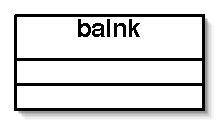
\includegraphics[width=0.4\textwidth]{figs/blank}
\end{center}
\caption{}
\label{fig:}
\end{figure}

This section describes the DnsQuery component, which is described by Figure~\ref{fig:}.  

The DnsQuery component encapsulates the NAT3-specific DNS logic needed by this application. It responds to error replies to questions for A resource records by generating questions for NAT3 records. If those are properly received, it asks the TunnelManager to set up a mapping. It will then construct a DNS response with an A record for this local mapping. It returns both this DNS response and the mapping itself to the resolver.

\subsection{Methods}

{\bf Public Methods}
\begin{itemize}
\item constructor: The constructor takes a socket address and a question packet and encapsulates them.
\item add\_response(): This method takes a parsed DNS packet that represents a response to a previous packet. The DnsQuery object then uses the data in this packet to create a ``next packet'' to send, encapsulating the high-level NAT3-specific DNS logic.
\item next\_packet(): This method returns a wire-encoded DNS message and a destination socket address representing the next packet to be sent.
\item get\_mapping(): This methods returns the mapping given by the TunnelManager to the DNS resolver if one has been made.
\item done(): True when a query has been completed.
\end{itemize}

{\bf Private Methods}
\begin{itemize}
\item get\_A\_RR(): Returns the first A resource record from the question section of the input packet, if one exists.
\end{itemize}

\subsection{Member Variables}
\begin{itemize}
\item m\_src: Socket address representing the source of the original packet.
\item m\_packet: Original DNS reply packet that was received from the caching resolver.
\item m\_fwd\_packet: Packet to be forwarded to the caching resolver or original questioner.
\item m\_orig\_error: Original error packet (i.e., NXDOMAIN) in case no NAT3 RR could be found.
\item m\_done: Flag used by done() method.
\end{itemize}
